\documentclass{beamer}
\usetheme{Boadilla}
\usepackage{tikz}
\usetikzlibrary{shapes.geometric,arrows, positioning, fit}

\title{Weekly Presentation}
\subtitle{Week 40}
\author{Martin Blaszczyk\\
        Edward Källstedt \\
        Albin Martinsson\\
        Måns Norell
        }
\institute{Luleå University of Technology}
\date{\today}

\begin{document}

\tikzstyle{computing} = [draw, rectangle, fill=white!50, rounded corners, node distance=2cm,
                    minimum height=3em]

\tikzstyle{io} = [rectangle, draw, trapezium right angle=110, rounded corners,
                  fill=red!20, node distance=1.9cm, minimum height=2.9em]

\tikzstyle{calculate} = [diamond, draw, trapezium right angle=110, rounded corners,
                  fill=green!20, node distance=1.9cm, minimum height=2.9em]

\tikzstyle{hardware} = [rectangle, draw, trapezium right angle=110, rounded corners,
                  fill=blue!20, node distance=1.9cm, minimum height=2.9em]

\tikzstyle{external} = [rectangle, draw, trapezium right angle=110, rounded corners,
                  fill=gray!20, node distance=1.9cm, minimum height=2.9em]
\tikzstyle{line} = [draw, -latex']

\tikzstyle{function} = [rectangle, draw, fill=green!20, node distance=1.9cm, minimum height=2.9em]
\tikzstyle{ros} = [circle, draw,
                  fill=gray!20, node distance=1.9cm, minimum height=2.9em]



\begin{frame}
    \titlepage
\end{frame}

\begin{frame}
    \frametitle{Overview}
    \tableofcontents
\end{frame}
%%%%%%%%%%%%%%%%%%%%%%%%%%%%%%%%%%%%%%%%%%%%%%%%%%%%%%%%%%%%%%%%
%%%%%%%%%%%%%%%%%%%%% Status %%%%%%%%%%%%%%%%%%%%%%%%
%%%%%%%%%%%%%%%%%%%%%%%%%%%%%%%%%%%%%%%%%%%%%%%%%%%%%%%%%%%%%%%%
\section{Status update}
\begin{frame}
    \subsection{Overall timetable}
    \frametitle{Overall timetable}
    \begin{table}
        \begin{tabular}{| l | c | c | c | c }

            Sep & Oct & Nov & Dec \\
            \hline \hline
            Concept generation & Evaluation & Evaluation &  \\
            \hline
            Theory & Prototyping & Evaluation & Finishing up \\
            \hline
            Simulation & Evaluation & Evaluation & \\
            \hline
            Prototyping & Final Design & Evaluation &  \\
            \hline

        \end{tabular}
    \end{table}
\end{frame}

\subsection{September planning}
\begin{frame}
    \frametitle{Time plan for September}
    \begin{table}
        \begin{tabular}{l | c | c | c | c }
        Subproject & Week 1 & Week 2 & Week 3 & Week 4 \\
        \hline \hline
            Arrowhead & Reading& Setup & API & Prototyping\\
            Movable base & Reading& Modeling & Simulation & Implementation\\
            Arm and grip  & Reading & Kinematics & Simulation& Prototyping\\
            Object detection & Reading & Testing & Prototyping & Evaluation\\
        \end{tabular}
    \end{table}
\end{frame}

%%%%%%%%%%%%%%%%%%%%%%%%%%%%%%%%%%%%%%%%%%%%%%%%%%%%%%%%%%%%%%%%%%%%%%%%%%
%%%%%%%%%%%%%%%%%%%%%%%%%%%% Engineering Problem %%%%%%%%%%%%%%%%%%%%%%%%%
%%%%%%%%%%%%%%%%%%%%%%%%%%%%%%%%%%%%%%%%%%%%%%%%%%%%%%%%%%%%%%%%%%%%%%%%%%
\section{Hardware}
\begin{frame}
    \subsection{New toys}
    \frametitle{New toys!}
    \begin{itemize}
        \item NVIDIA Jetson Nano
        \item Cameras
        \item Dynamixel Smart motors
        \item Screws, cables and other goodies
    \end{itemize}
\end{frame}

\begin{frame}
    \frametitle{NVIDIA Jetson Nano}
    \begin{columns}
        \begin{column}[]{0.5\textwidth}
            \begin{itemize}
                \item Runs Ubuntu
                \item Two camera ports (CSI)
                \item More powerful GPU than RPi
            \end{itemize}
        \end{column}

        \begin{column}[]{0.5\textwidth}
            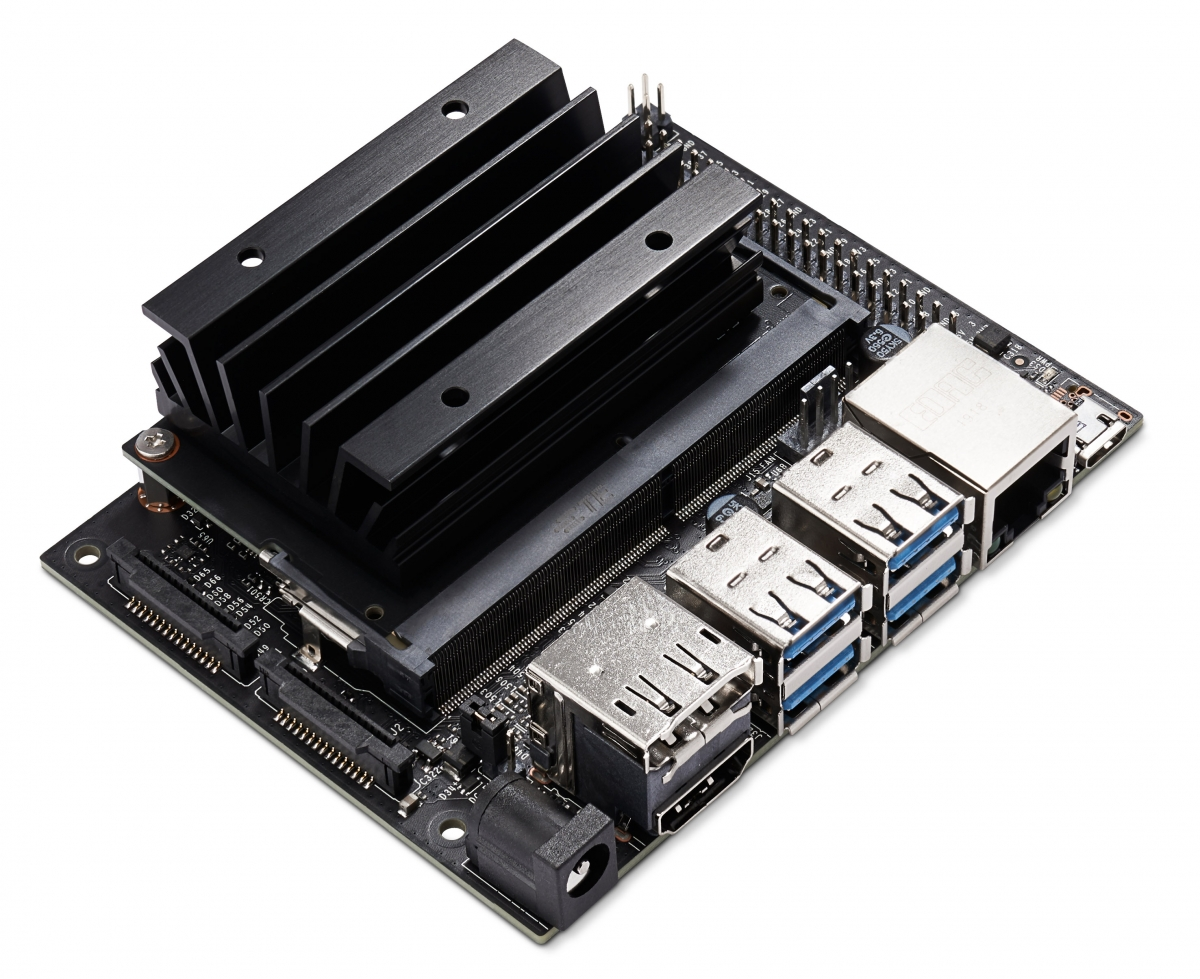
\includegraphics[width=\textwidth]{img/nvidia.jpg}
        \end{column}
    \end{columns}


\end{frame}
\begin{frame}
    \frametitle{Cameras}
    \begin{columns}
        \begin{column}[]{0.5\textwidth}
            \begin{itemize}
                \item Compatible with NVIDIA and RPi
                \item Small package
                \item 8 megapixels
                \item Video:
                \begin{itemize}
                    \item 1080p @ 30 fps
                    \item 720p @ 60fps
                \end{itemize}

            \end{itemize}
        \end{column}

        \begin{column}[]{0.5\textwidth}
            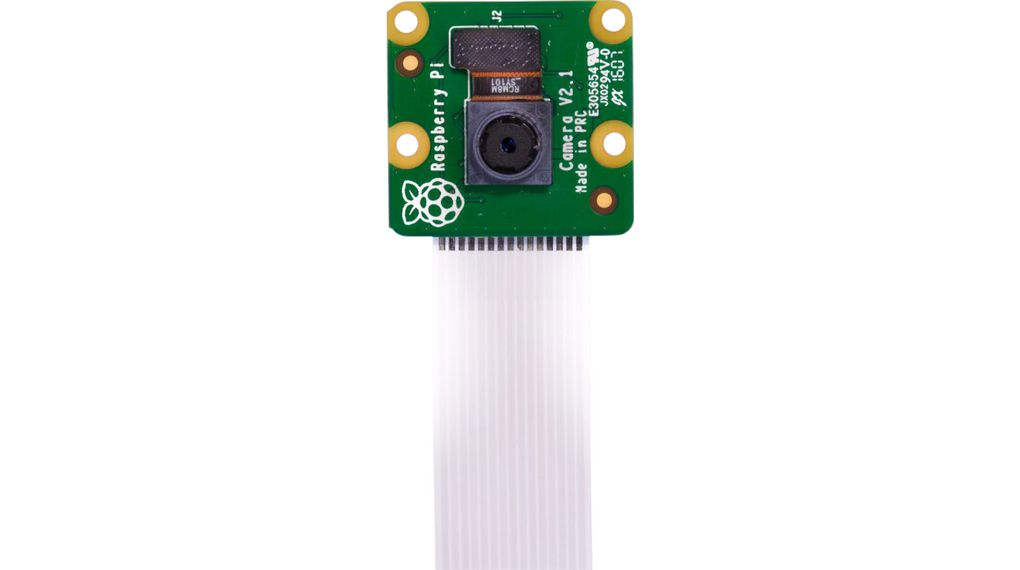
\includegraphics[width=\textwidth]{img/camera.jpg}
        \end{column}
    \end{columns}
\end{frame}
\begin{frame}
    \frametitle{Dynamixel Smart Motors}
    \begin{columns}
        \begin{column}[]{0.5\textwidth}
            \begin{itemize}
                \item Connects in series
                \item Angle and wheel mode
                \item Feedback
            \end{itemize}
        \end{column}

        \begin{column}[]{0.5\textwidth}
            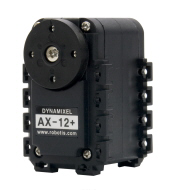
\includegraphics[width=\textwidth]{img/dynamixel.png}
        \end{column}
    \end{columns}
\end{frame}
\begin{frame}
    \frametitle{Hardware}
    \centering
    \resizebox{7.0cm}{!}{
    \begin{tikzpicture}
        [align=center, node distance=1em, auto]

        \node [computing] (pc) {Arrowhead PC};
        \node [computing, below= of pc] (nvidia) {NVIDIA};
        \node [io, right= of nvidia] (battery) {Battery};
        \node [computing, right= of pc] (factory) {Factory};
        \node [io, below of= nvidia] (cameras) {Cameras};
        \node [io, right= 1em of cameras] (motors) {Motors};
        \node [io, left= 1em of cameras] (distance_sensors) {Distance sensors};
        \node [io, below= of motors] (arm) {Robot arm};
        \node [io, right= 1em of arm] (base) {Base};
        \node [rectangle=white, left= 5em of nvidia] (robot) {Robot};

        \path [line] (nvidia)--(cameras);
        \path [line] (battery)--(nvidia);
        \path [line] (battery)--(motors);
        \path [line] (nvidia)--(motors);
        \path [line] (nvidia)--(distance_sensors);
        \draw[->] (factory) -- (pc);
        \draw[<->] (pc) -- (nvidia);
        \draw[->] (motors) -- (arm);
        \draw[->] (motors) -- (base);
        \node [draw=black, dashed, fit= (nvidia) (battery) (distance_sensors)
        (cameras) (motors) (base) (arm)]{};

    \end{tikzpicture}
    }
\end{frame}
\section{Machine vision}
\subsection{Flows}
\begin{frame}
    \frametitle{Object detection}
    \begin{itemize}
        \item Line detection now works
        \item Testing cameras and real time performance on NVIDIA
        \item Will be using two cameras.
        \begin{itemize}
            \item Front facing
            \item Downwards facing
        \end{itemize}
    \end{itemize}
\end{frame}

\begin{frame}
    \frametitle{Machine vision}
    \centering
    \resizebox{7.0cm}{!}{
    \begin{tikzpicture}

        \node [hardware] (fcamera) {Front facing camera};
        \node [hardware, right= of fcamera] (dcamera) {Down facing camera};
        \path (fcamera) -- (dcamera) coordinate[midway] (aux);
        \node [computing, below= of aux] (opencv) {OpenCV};
        \node [function, below= of opencv] (qr) {QR-codes};
        \node [function, left= of qr] (line_follow) {Line follower};
        \node [function, right= of qr] (obj_detection) {Object detection};
        \coordinate [below= of line_follow] (aux3);
        \coordinate [below= of obj_detection] (aux4);
        \node [external, left= 1em of aux4] (cylinder) {Cylinder};
        \node [external, right= 1em of aux4] (factory) {Factory};
        \coordinate [below= of opencv] (aux5);



        \draw [->] (fcamera)|- node[midway, fill=white] {frame} (opencv);
        \draw [->] (dcamera)|- node[midway, fill=white] {frame} (opencv);
        \draw [->] (qr) -- node[midway, fill=white] {ID} (obj_detection);
        \draw [->] (qr) -- node[midway, fill=white] {Nav} (line_follow);
        \draw [<-] (factory.north) -- (factory|-obj_detection.south);
        \draw [<-] (cylinder.north) -- (cylinder|-obj_detection.south);
        \draw [->] (opencv) -- (aux5) -| (obj_detection);
        \draw [->] (aux5) -- (qr);
        \draw [->] (aux5) -| (line_follow);

    \end{tikzpicture}
    }
\end{frame}

\begin{frame}
    \frametitle{OpenCV}
    \centering
    \resizebox{7.0cm}{!}{
    \begin{tikzpicture}
        [align=center, auto]
        \node [io] (rgb) {RGB Frame};
        \node [function, below= 2em of rgb] (rgb2hsv) {RGB to HSV};
        \node [io, below= 2em of rgb2hsv] (hsv) {HSV Frame};
        \node [function, below= of hsv] (qr) {QR-scanner};
        \node [function, right= 10em of qr] (mass) {Calculate center \\of mass};
        \node [function, left= 10em of qr] (cylinder) {Localize cylinder};
        \node [io, below= 1em of cylinder] (ccoordinate) {Cylinder \\position [x,y,z]};
        \node [io, below= 1em of mass] (coordinate) {Center of line [x,y]};
        \node [io, below= 1em of coordinate] (angle) {Angle [deg]};
        \coordinate [below= of qr] (aux1);
        \node [io, left= 1em of aux1] (id) {Identification};
        \node [io, right= 1em of aux1] (position) {Position in space \\ (x,y) };
        \node [io, below= 1em of id] (action) {Action at QR};

        \draw [->] (rgb) -- (rgb2hsv) -- (hsv);
        \coordinate [below= of hsv] (aux2);
        \draw [->] (hsv) -- (aux2) -| (mass);
        \draw [->] (aux2) -| (cylinder);
        \draw [->] (aux2) -- (qr);
        \draw [->] (mass) -- (coordinate) -- (angle);
        \draw [->] (cylinder) -- (ccoordinate);
        \draw [->] (qr) -| (id);
        \draw [->] (qr) -| (position);
        \draw [->] (id) -- (action);

        \node [ros, below= 15emof qr] (ros) {ROS publish};

        \draw [->] (position.south) -- (ros);
        \draw [->] (action.south) -- (ros);
        \draw [->] (ccoordinate.south) -- (ros);
        \draw [->] (coordinate.south west) -- (ros);
        \draw [->] (angle.south west) -- (ros);
    \end{tikzpicture}
    }
\end{frame}

\subsection{Line following algorithm}

\begin{frame}
    \frametitle{Line following algorithm}
    \begin{itemize}
	    \item \url{https://www.youtube.com/watch?v=TdtPIdipSBY}
    \end{itemize}
\end{frame}
\begin{frame}
    \frametitle{Line following algorithm - Procedure}
    \begin{itemize}
	    \item HSV mask to select color space
        \item Crop image into horizontal slice
        \item Calculate image moment on slice to extract centroid
        \item Calculate angle between robot base and line
    \end{itemize}
\end{frame}
\begin{frame}
    \frametitle{Line following algorithm - Optimization}
    \begin{itemize}
	    \item Only search adjacent to previous line position
        \item Implement CUDA support
    \end{itemize}
\end{frame}
\begin{frame}
    \frametitle{CV - What's next?}
    \begin{itemize}
	    \item Implement QR code functionality
        \item Finalize API consumed by other parts of the system
        \item Clean up code and implement proper configuration capabilities
    \end{itemize}
\end{frame}
\section{Movable base}
\begin{frame}{Movable Base}
    What has been done
    \begin{itemize}
        \item Mathematical model
        \item Controller selection
        \item Some simulations (more work needs to be done)
    \end{itemize}
 \end{frame}

 %%%%%%%%%%%%%%%% new page %%%%%%%%%%%%%%%%%%%%%%


\begin{frame}{Mathematical Model}
    \begin{columns}
    \begin{column}[]{0.5\textwidth}
    Actuators:
        \begin{itemize}
            \item The motors of the left and right track ($v_L,v_R$)
        \end{itemize}
    Parameters to Control:
    \begin{itemize}
        \item The angle to a coloured line ($\theta$)
    \end{itemize}
    \end{column}
    \begin{column}[]{0.5\textwidth}
    \begin{figure}
        \centering
        \includegraphics[width=0.5\textwidth]{model_of_base.png}
        \caption{Model of base}
        \label{fig:my_label}
    \end{figure}
    \end{column}
    \end{columns}
    \end{frame}
    
    
    %%%%%%%%%%%%%%%% new page %%%%%%%%%%%%%%%%%%%%%%
    
    
    \begin{frame}{Mathematical Model}
    Given the $v_L$, $v_R$ and $\theta$ we can calculate
        \begin{itemize}
            \item $\overline{v}=||v||*(-\cos{\theta}*\hat{i}+\sin{\theta}*\hat{j})$
            \item $\overline{L}=\int \overline{v}$
            %\item $\theta=\frac{sin^{-1}(L_{Ly} - L_{Ry)}}{2 r}$ (r: Length from center of base to center of track)
            \item $\dot{\theta}=\frac{v_R-v_L}{2 r}$
        \end{itemize}
    \end{frame}
    
    
    %%%%%%%%%%%%%%%% new page %%%%%%%%%%%%%%%%%%%%%%
    
    
    \begin{frame}{Controller Choice}
    
        The robot will use two \textbf{PD} controllers for the line following
        
    \end{frame}
    
    %%%%%%%%%%%%%%%% new page %%%%%%%%%%%%%%%%%%%%%%
    
    
    \begin{frame}{Controller Choice}
    
        The robot will use two \textbf{PD} controllers for the line following
        
        \begin{itemize}
            \item Simple \textbf{P} controller is not smooth enough
            \item \textbf{PID} is more likely to overshoot
        \end{itemize}
        
    \end{frame}
    
    %%%%%%%%%%%%%%%% new page %%%%%%%%%%%%%%%%%%%%%%
    
    \begin{frame}{Simulations}
    \begin{columns}
    \begin{column}[]{0.5\textwidth}
    \begin{figure}
        \centering
        \includegraphics[width=\textwidth]{Robot_displacement.png}
        \caption{Angle from line}
        \label{fig:my_label}
    \end{figure}
    \end{column}
    \begin{column}[]{0.5\textwidth}
    \begin{figure}
        \centering
        \includegraphics[width=\textwidth]{Motor_speed.png}
        \caption{Motor speed for left and right motor}
        \label{fig:my_label}
    \end{figure}
    \end{column}
    \end{columns}
        
    \end{frame}
    
    
    %%%%%%%%%%%%%%%% new page %%%%%%%%%%%%%%%%%%%%%%
    
    
    \begin{frame}{Simulations}
    To be done
    
    \begin{itemize}
        \item Import real values from the motors and base for applicable simulations
        \item Insert boundaries for control signals
    \end{itemize}
    
    \end{frame}

\subsection{Arrowhead}

\begin{frame}
    \frametitle{Arrowhead}
    

\end{frame}

\begin{frame}
    \begin{center}
        \Huge Questions?
    \end{center}
\end{frame}



\end{document}
